\documentclass[12pt,a4paper]{article}
\usepackage[utf8]{vietnam}
\usepackage{amsmath,amssymb}
\usepackage{tabularx}
\usepackage{graphicx}
\usepackage{tikz}
\usetikzlibrary{calc,arrows.meta}
\usepackage{xcolor}
\usepackage{enumitem}
\usepackage{fancyhdr}
\usepackage[top=1.0cm, bottom=1.0cm, left=1.2cm, right=1.2cm]{geometry}
\usepackage[dethi]{ex_test}
\SAOPTN{widthSA=2.6,heightSA=0.62}

\setlength{\headheight}{15pt}
\setlength{\parskip}{0pt}

% Dòng kẻ chấm mờ chuẩn viết tay
\newcommand{\dongke}[1]{%
  \begingroup%
  \setlength{\parskip}{0pt}%
  \baselineskip=18.5pt%
  \vspace{1.0mm}%
  \foreach \i in {1,...,#1}{%
    \noindent{\color{gray!60}\dotfill}\par%
  }%
  \vspace{0.6mm}%
  \endgroup%
}

\pagestyle{fancy}
\fancyhf{}
\rhead{\textit{Môn Toán 7 -- Đề số 9}}
\lhead{\textit{Bộ đề ôn tập Giữa học kì I}}
\cfoot{\thepage}

\begin{document}

% --- KHUNG TIÊU ĐỀ ĐỀ THI ---
\noindent
\begin{tabularx}{\linewidth}{X r}
\textbf{TRƯỜNG THCS: \dotfill} & \textbf{ĐỀ KIỂM TRA ĐỊNH KỲ GIỮA HỌC KỲ I} \\
\textbf{Họ và tên: \dotfill} & \textbf{NĂM HỌC 2026 -- 2027} \\
\textbf{Lớp: \dotfill \quad SBD: \dotfill} & \textbf{Môn: TOÁN 7} \\
& \textit{Thời gian làm bài: 90 phút (không kể thời gian phát đề)}
\end{tabularx}

\vspace{1mm}
\noindent
\begin{tabularx}{\linewidth}{|p{3.5cm}|X|}
\hline
\centering\textbf{Điểm số} & \centering\textbf{Lời nhận xét của thầy cô giáo} \tabularnewline
\rule{0pt}{1.0cm} & \\
\hline
\end{tabularx}

\vspace{1.5mm}
\begin{center}
\textbf{\large ĐỀ SỐ 9}
\end{center}

\noindent\textbf{\large PHẦN I. CÂU TRẮC NGHIỆM NHIỀU PHƯƠNG ÁN LỰA CHỌN (3,0 điểm)}

\textit{Thí sinh trả lời từ câu 1 đến câu 12. Mỗi câu hỏi chỉ chọn một phương án đúng nhất và ghi vào bảng đáp án.}

\vspace{1mm}
\begin{ex}
Trong các phân số sau, phân số nào biểu diễn số hữu tỉ $-0{,}5$?
\choice
{$\dfrac{1}{2}$}
{\True $-\dfrac{1}{2}$}
{$\dfrac{3}{5}$}
{$-\dfrac{3}{5}$}
\end{ex}

\begin{ex}
\immini{
Quan sát trục số sau. Điểm $A$ biểu diễn số hữu tỉ nào?
\choice
{$\dfrac{3}{5}$}
{$-\dfrac{3}{4}$}
{$-3$}
{\True $-\dfrac{3}{5}$}
}{
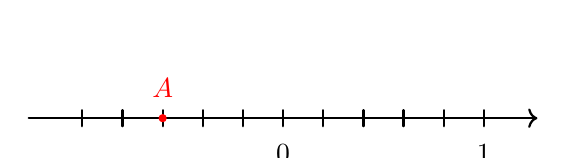
\begin{tikzpicture}[scale=0.85, line cap=round, line join=round]
    \draw[thick, ->] (-3.8, 0) -- (3.8, 0);
    \foreach \x in {-3.0, -2.4, -1.8, -1.2, -0.6, 0, 0.6, 1.2, 1.8, 2.4, 3.0} {
        \draw[thick] (\x, 0.12) -- (\x, -0.12);
    }
    \node[below=3pt] at (0, -0.12) {$0$};
    \node[below=3pt] at (3.0, -0.12) {$1$};
    \filldraw[red] (-1.8, 0) circle (1.5pt) node[above=4pt, red, font=\bfseries] {$A$};
\end{tikzpicture}
}
\end{ex}

\begin{ex}
Phép tính nào sau đây là không đúng?
\choice
{$(x^3)^4 = x^{12}$}
{$x^{18} : x^6 = x^{12}$ ($x \neq 0$)}
{\True $x^2 \cdot x^6 = x^{12}$}
{$x^4 \cdot x^8 = x^{12}$}
\end{ex}

\begin{ex}
Kết quả của phép tính $2^2 \cdot 2^5$ là:
\choice
{$2^{10}$}
{$2^3$}
{$2^5$}
{\True $2^7$}
\end{ex}

\begin{ex}
Một hình vuông có diện tích $81\text{ cm}^2$. Độ dài cạnh hình vuông đó là:
\choice
{$81\text{ cm}$}
{\True $9\text{ cm}$}
{$-9\text{ cm}$}
{$\pm 9\text{ cm}$}
\end{ex}

\begin{ex}
Làm tròn số $1{,}3781$ với độ chính xác $0{,}005$ được kết quả là:
\choice
{$1{,}37$}
{$1{,}4$}
{$1$}
{\True $1{,}38$}
\end{ex}

\begin{ex}
Trong các hình sau, hình nào không phải là hình lăng trụ đứng tứ giác?
\begin{center}
\includegraphics[width=10.5cm]{crops/test_p42_xref3051.png}
\end{center}
\choice
{Hình 1}
{\True Hình 2}
{Hình 3}
{Hình 4}
\end{ex}

\begin{ex}
Thực hiện phép tính $M = \dfrac{13}{31} + \dfrac{4}{15} + \dfrac{18}{31} + \dfrac{2024}{2025} - \dfrac{19}{15}$, ta được kết quả là:
\choice
{\True $M = \dfrac{2024}{2025}$}
{$M = -\dfrac{2024}{2025}$}
{$M = 1$}
{$M = 0$}
\end{ex}

\begin{ex}
\immini{
Tia phân giác của $\widehat{xOm}$ và $\widehat{yOn}$ lần lượt là:
\choice
{\True $Ok$ và $Ou$}
{$Ox$ và $Oy$}
{$Ou$ và $Om$}
{$Ok$ và $On$}
}{
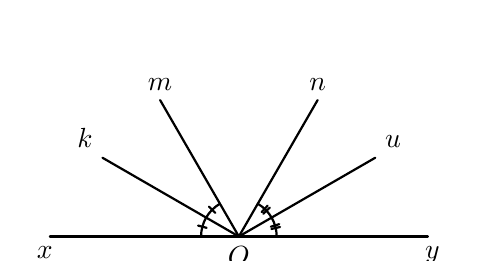
\begin{tikzpicture}[scale=0.8, line cap=round, line join=round]
    \coordinate (O) at (0, 0);
    \coordinate (x) at (-2.8, 0);
    \coordinate (y) at (2.8, 0);
    \coordinate (k) at ({2.5*cos(150)}, {2.5*sin(150)});
    \coordinate (m) at ({2.5*cos(120)}, {2.5*sin(120)});
    \coordinate (n) at ({2.5*cos(60)}, {2.5*sin(60)});
    \coordinate (u) at ({2.5*cos(30)}, {2.5*sin(30)});

    \draw[thick] (-3.0, 0) -- (3.0, 0);
    \draw[thick] (O) -- (k);
    \draw[thick] (O) -- (m);
    \draw[thick] (O) -- (n);
    \draw[thick] (O) -- (u);

    \node[below] at (O) {$O$};
    \node[below left] at (-2.8, 0) {$x$};
    \node[below right] at (2.8, 0) {$y$};
    \node[above left] at (k) {$k$};
    \node[above] at (m) {$m$};
    \node[above] at (n) {$n$};
    \node[above right] at (u) {$u$};

    % Arcs for xOk and kOm
    \draw[thick] (O) ++(180:0.6) arc (180:150:0.6);
    \draw[thick] (O) ++(150:0.6) arc (150:120:0.6);
    \draw[thick] ($(O)+(165:0.53)$) -- ($(O)+(165:0.67)$);
    \draw[thick] ($(O)+(135:0.53)$) -- ($(O)+(135:0.67)$);

    % Arcs for yOu and uOn
    \draw[thick] (O) ++(0:0.6) arc (0:30:0.6);
    \draw[thick] (O) ++(30:0.6) arc (30:60:0.6);
    \draw[thick] ($(O)+(13:0.53)$) -- ($(O)+(13:0.67)$);
    \draw[thick] ($(O)+(17:0.53)$) -- ($(O)+(17:0.67)$);
    \draw[thick] ($(O)+(43:0.53)$) -- ($(O)+(43:0.67)$);
    \draw[thick] ($(O)+(47:0.53)$) -- ($(O)+(47:0.67)$);
\end{tikzpicture}
}
\end{ex}

\begin{ex}
Tổng ba góc trong một tam giác luôn bằng:
\choice
{$90^\circ$}
{$120^\circ$}
{\True $180^\circ$}
{$360^\circ$}
\end{ex}

\begin{ex}
Hai đường thẳng $xy$ và $x'y'$ cắt nhau tại $O$. Biết $\widehat{xOx'} = 70^\circ$. $Ot$ là tia phân giác của $\widehat{xOx'}$, $Ot'$ là tia đối của tia $Ot$. Tính số đo góc $\widehat{yOt'}$?
\choice
{\True $35^\circ$}
{$70^\circ$}
{$145^\circ$}
{$110^\circ$}
\end{ex}

\begin{ex}
Đối với biểu thức không có dấu ngoặc và chỉ có các phép tính: cộng, trừ, nhân, chia, lũy thừa, thì thứ tự thực hiện phép tính đúng là:
\choice
{\True Lũy thừa $\to$ Nhân và chia $\to$ Cộng và trừ}
{Nhân và chia $\to$ Lũy thừa $\to$ Cộng và trừ}
{Cộng và trừ $\to$ Nhân và chia $\to$ Lũy thừa}
{Lũy thừa $\to$ Cộng và trừ $\to$ Nhân và chia}
\end{ex}


\vspace{1mm}
\noindent\textbf{BẢNG TRẢ LỜI TRẮC NGHIỆM PHẦN I:}
\begin{center}
\begin{tabular}{|c|c|c|c|c|c|c|c|c|c|c|c|c|}
\hline
\textbf{Câu} & \textbf{1} & \textbf{2} & \textbf{3} & \textbf{4} & \textbf{5} & \textbf{6} & \textbf{7} & \textbf{8} & \textbf{9} & \textbf{10} & \textbf{11} & \textbf{12} \\
\hline
\textbf{Chọn} & \rule{0pt}{0.55cm} & & & & & & & & & & & \\
\hline
\end{tabular}
\end{center}
\vspace{1mm}

\setcounter{ex}{0}
\noindent\textbf{\large PHẦN II. CÂU TRẮC NGHIỆM ĐÚNG SAI (2,0 điểm)}

\textit{Thí sinh trả lời câu 1 và câu 2. Trong mỗi ý a), b), c), d) ở mỗi câu, thí sinh chọn đúng hoặc sai.}

\vspace{1mm}
\begin{ex}
Cho biểu thức $P = \left(-\dfrac{2}{3}\right)^2 + \dfrac{5}{9} : \left(-\dfrac{5}{3}\right) - \left|-\dfrac{1}{3}\right|$. Xét tính đúng sai của các mệnh đề sau:
\choiceTF
{\True Giá trị của lũy thừa $\left(-\dfrac{2}{3}\right)^2$ bằng $\dfrac{4}{9}$}
{\True Kết quả của phép chia $\dfrac{5}{9} : \left(-\dfrac{5}{3}\right)$ bằng $-\dfrac{1}{3}$}
{Giá trị tuyệt đối $\left|-\dfrac{1}{3}\right|$ bằng $-\dfrac{1}{3}$}
{\True Giá trị của biểu thức $P$ bằng $-\dfrac{2}{9}$}
\end{ex}

\begin{ex}
Cho $\Delta ABC = \Delta DEF$ với $AB = 8\text{ cm}, BC = 6\text{ cm}, DF = 10\text{ cm}$; $\widehat{B} = 90^\circ, \widehat{C} = 53^\circ$. Xét tính đúng sai của các mệnh đề sau:
\choiceTF
{Số đo góc $E$ bằng $53^\circ$}
{\True Độ dài cạnh $AC = 10\text{ cm}$}
{Độ dài cạnh $EF = 8\text{ cm}$}
{\True Tổng số đo $\widehat{D} + \widehat{F} = 90^\circ$}
\end{ex}


\noindent\textbf{BẢNG TRẢ LỜI PHẦN II:}
\begin{center}
\begin{tabular}{|c|c|c|c|c||c|c|c|c|c|}
\hline
\textbf{Câu 1} & \textbf{a)} & \textbf{b)} & \textbf{c)} & \textbf{d)} & \textbf{Câu 2} & \textbf{a)} & \textbf{b)} & \textbf{c)} & \textbf{d)} \\
\hline
\textbf{Đ/S} & \rule{0pt}{0.5cm} & & & & \textbf{Đ/S} & & & & \\
\hline
\end{tabular}
\end{center}
\vspace{1mm}

\setcounter{ex}{0}
\noindent\textbf{\large PHẦN III. CÂU HỎI TRẢ LỜI NGẮN (1,0 điểm)}

\textit{Thí sinh trả lời câu 1 và câu 2. Điền kết quả vào ô trống.}

\vspace{1mm}
\begin{ex}
Tìm số hữu tỉ $x$, biết: $\dfrac{2}{3} + \dfrac{1}{3} : x = -\dfrac{1}{6}$. \shortans{$-\dfrac{2}{5}$}
\end{ex}

\begin{ex}
\immini{
Cho hình vẽ sau, biết $\widehat{CFE} = 60^\circ$ và $\widehat{E}_1 = 120^\circ$. Số đo của góc $\widehat{FEB}$ bằng bao nhiêu độ?
\vspace{1mm}
\hfill\shortans{$60^\circ$}
}{
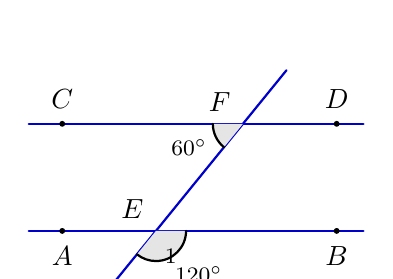
\begin{tikzpicture}[scale=0.85, line cap=round, line join=round]
    \coordinate (E) at (1.1, 0);
    \coordinate (F) at (2.4, 1.6);

    \draw[thick, blue!80!black] (-0.8, 1.6) -- (4.2, 1.6);
    \draw[thick, blue!80!black] (-0.8, 0) -- (4.2, 0);

    \filldraw[black] (-0.3, 1.6) circle (1pt) node[above=2pt] {$C$};
    \filldraw[black] (3.8, 1.6) circle (1pt) node[above=2pt] {$D$};
    \filldraw[black] (-0.3, 0) circle (1pt) node[below=2pt] {$A$};
    \filldraw[black] (3.8, 0) circle (1pt) node[below=2pt] {$B$};

    \draw[thick, blue!80!black] ($(E)!-0.5!(F)$) -- ($(F)!-0.5!(E)$);

    \node[above left=1pt] at (E) {$E$};
    \node[above left=1pt] at (F) {$F$};

    % Angle CFE = 60 deg
    \fill[gray!20] (F) -- ++(180:0.45) arc (180:231:0.45) -- cycle;
    \draw[thick] (F) ++(180:0.45) arc (180:231:0.45);
    \node[font=\footnotesize, below left=1pt] at ($(F)+(-0.35, -0.05)$) {$60^\circ$};

    % Angle E1 = 120 deg
    \fill[gray!20] (E) -- ++(0:0.45) arc (0:-129:0.45) -- cycle;
    \draw[thick] (E) ++(0:0.45) arc (0:-129:0.45);
    \node[font=\footnotesize, below=2pt] at ($(E)+(0.22, -0.05)$) {$1$};
    \node[font=\footnotesize, below right=1pt] at ($(E)+(0.1, -0.35)$) {$120^\circ$};
\end{tikzpicture}
}
\end{ex}


\newpage
\setcounter{ex}{0}
\noindent\textbf{\large PHẦN IV. TỰ LUẬN (4,0 điểm)}

\textit{Thí sinh trình bày chi tiết lời giải vào giấy làm bài.}

\vspace{1mm}
\begin{ex}
Thực hiện phép tính (tính hợp lí nếu có):
\begin{enumerate}[label=\textbf{\alph*)}, leftmargin=0.8cm, itemsep=1pt]
\item $\dfrac{-4}{12} + \dfrac{14}{21}$;
\item $\dfrac{8}{3} \cdot \dfrac{9}{4}$.
\end{enumerate}
\end{ex}
\vspace{1.5mm}

\begin{ex}
Tìm $x$, biết:
\begin{enumerate}[label=\textbf{\alph*)}, leftmargin=0.8cm, itemsep=1pt]
\item $x - \dfrac{2}{3} = \dfrac{5}{6}$;
\item $(1 - x)^2 = \dfrac{4}{9}$.
\end{enumerate}
\end{ex}
\vspace{1.5mm}

\begin{ex}
\immini{
Cho hình vẽ, biết rằng: $\widehat{mAx} = 40^\circ, \widehat{ABt} = 140^\circ$.
\begin{enumerate}[label=\textbf{\alph*)}, leftmargin=0.8cm, itemsep=1pt]
\item Tính số đo góc $\widehat{mAy}$;
\item Chứng tỏ $xy \parallel zt$;
\item Tia phân giác của góc $\widehat{xAB}$ cắt đường thẳng $zt$ tại điểm $C$. Tính số đo $\widehat{ACB}$.
\end{enumerate}
}{
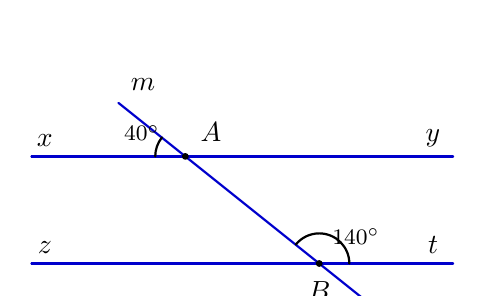
\begin{tikzpicture}[scale=0.85, line cap=round, line join=round]
    \coordinate (A) at (1.8, 1.6);
    \coordinate (B) at (3.8, 0);

    \draw[thick, blue!80!black] (-0.5, 1.6) -- (5.8, 1.6);
    \draw[thick, blue!80!black] (-0.5, 0) -- (5.8, 0);

    \node[above] at (-0.3, 1.6) {$x$};
    \node[above] at (5.5, 1.6) {$y$};
    \node[above] at (-0.3, 0) {$z$};
    \node[above] at (5.5, 0) {$t$};

    % Line mB
    \draw[thick, blue!80!black] ($(A)!-0.5!(B)$) -- ($(B)!-0.4!(A)$);

    \node[above right=1pt] at ($(A)!-0.5!(B)$) {$m$};
    \filldraw[black] (A) circle (1.2pt) node[above right=2pt] {$A$};
    \filldraw[black] (B) circle (1.2pt) node[below=3pt] {$B$};

    % Angle mAx = 40 deg
    \draw[thick] (A) ++(180:0.45) arc (180:141:0.45);
    \node[font=\footnotesize] at ($(A)+(-0.65, 0.35)$) {$40^\circ$};

    % Angle ABt = 140 deg
    \draw[thick] (B) ++(0:0.45) arc (0:141:0.45);
    \node[font=\footnotesize] at ($(B)+(0.55, 0.4)$) {$140^\circ$};
\end{tikzpicture}
}
\end{ex}
\vspace{1.5mm}

\begin{ex}
Cho biểu thức $M = \dfrac{1}{2^2} + \dfrac{1}{3^2} + \dfrac{1}{3^4} + \dfrac{1}{3^6} + \dots + \dfrac{1}{3^{802}}$. Chứng minh rằng $M < \dfrac{3}{8}$.
\end{ex}
\vspace{1.5mm}


\begin{center}
\rule{4cm}{0.4pt}\\
\textit{--- HẾT ---}
\end{center}
\end{document}
